%%%%%%%%%%%%%%%%%%%%%%%%%%%%%%%%%%%%%%%%%%%%%%%%%%%%%%%%%%%%%%%%%%%%%%
%%  Copyright by Wenliang Du.                                       %%
%%  This work is licensed under the Creative Commons                %%
%%  Attribution-NonCommercial-ShareAlike 4.0 International License. %%
%%  To view a copy of this license, visit                           %%
%%  http://creativecommons.org/licenses/by-nc-sa/4.0/.              %%
%%%%%%%%%%%%%%%%%%%%%%%%%%%%%%%%%%%%%%%%%%%%%%%%%%%%%%%%%%%%%%%%%%%%%%

% *******************************************
% SECTION
% *******************************************
\section{Code Compilation}
\label{sidechannel:sec:compilation}


\paragraph{For Ubuntu 16.04 OS.}
For most of our tasks, you need to add \texttt{-march=native}
flag when compiling the code with
\texttt{gcc}. The \texttt{march} flag tells the compiler to enable all
instruction subsets supported by the local machine.
For example, we compile \texttt{myprog.c} using the following command:

\begin{lstlisting}
$ gcc -march=native -o myprog myprog.c
\end{lstlisting}

\paragraph{For Ubuntu 20.04 OS.}
On Ubuntu 20.04 OS, including the \texttt{-march=native} option may 
cause errors to some computers. From our debugging effort,
it seemed this option was no longer needed. Therefore, if you 
do encounter errors due to this option, try the compilation
without using the option:

\begin{lstlisting}
$ gcc -o myprog myprog.c
\end{lstlisting}




% *******************************************
% SECTION
% ******************************************* 
\section{Tasks 1 and 2: Side Channel Attacks via CPU Caches}

Both the Meltdown and Spectre attacks use CPU cache as a side channel to steal
a protected secret. The technique used in this side-channel attack is called 
FLUSH+RELOAD~\cite{Yarom2014}. 
We will study this technique first. The code developed in these two tasks will be 
used as a building block in later tasks. 


A CPU cache is a hardware cache used by the CPU of a computer 
to reduce the average cost (time or energy) to access
data from the main memory. Accessing data from CPU cache is much faster
than accessing from the main memory. When data are fetched from the main memory, they
are usually cached by the CPU, so if the same data are used again, the access
time will be much faster. Therefore, when a CPU needs to access some data, it
first looks at its caches. If the data is there (this is called cache hit), 
it will be fetched directly from there. If the data is not there (this is
called miss), the CPU will go to the main memory to get the data. The time 
spent in the latter case is significant longer. Most modern CPUs have
CPU caches. 



\begin{figure}[htb]
\centering
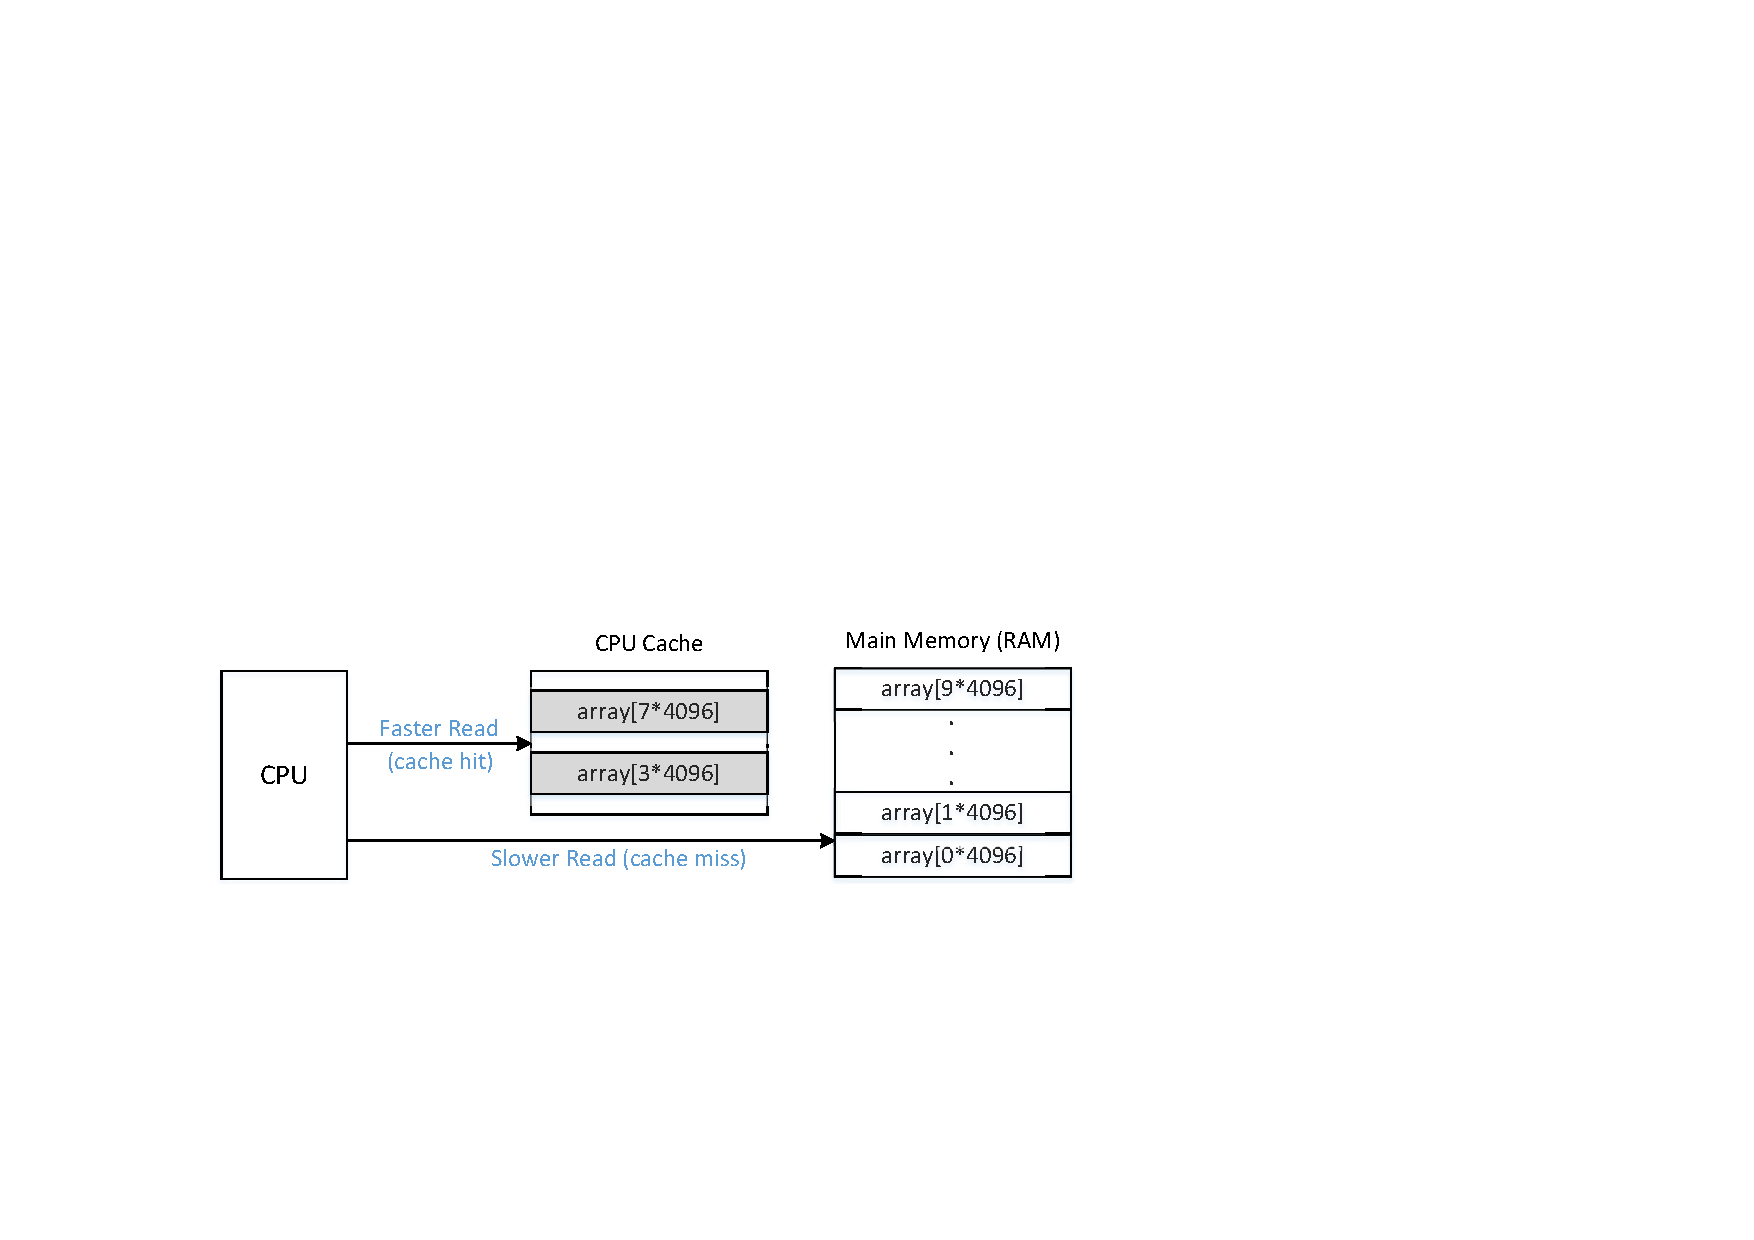
\includegraphics[width=0.9\textwidth]{\sideChannelFigs/cachehitmiss.pdf}
\caption{Cache hit and miss}
\label{sidechannel:fig:cachehitmiss}
\end{figure}


\subsection{Task 1: Reading from Cache versus from Memory}

The cache memory is used to provide data to the high speed processors at a faster speed. The
cache memories are very fast compared to the main memory. 
Let us see the time difference. In the following code (\texttt{CacheTime.c}), we 
have an array of size \texttt{10*4096}. We first access two of its elements,
\texttt{array[3*4096]} and \texttt{array[7*4096]}. Therefore, the pages 
containing these two elements will be cached. We then
read the elements from \texttt{array[0*4096]} to \texttt{array[9*4096]} and measure 
the time spent in the memory reading.
Figure~\ref{sidechannel:fig:cachehitmiss} illustrates the difference. 
In the code, Line \ding{192} reads the CPU's
timestamp (TSC) counter before the memory read, while Line \ding{193}
reads the counter after the memory read. Their difference is the time (in terms of number of
CPU cycles) spent in the memory read.  It should be noted that 
caching is done at the cache block level, not at the byte level. A typical cache block size 
is 64 bytes. We use \texttt{array[k*4096]}, so no two elements used in 
the program fall into the same cache block. 


\begin{lstlisting}[caption=\texttt{CacheTime.c}]
#include <emmintrin.h>
#include <x86intrin.h>

uint8_t array[10*4096];

int main(int argc, const char **argv) {
  int junk=0;
  register uint64_t time1, time2;
  volatile uint8_t *addr;
  int i;
  
  // Initialize the array
  for(i=0; i<10; i++) array[i*4096]=1;

  // FLUSH the array from the CPU cache
  for(i=0; i<10; i++) _mm_clflush(&array[i*4096]);

  // Access some of the array items
  array[3*4096] = 100;
  array[7*4096] = 200;

  for(i=0; i<10; i++) {
    addr = &array[i*4096];
    time1 = __rdtscp(&junk);                  (*@\ding{192}@*)
    junk = *addr;
    time2 = __rdtscp(&junk) - time1;          (*@\ding{193}@*)
    printf("Access time for array[%d*4096]: %d CPU cycles\n",i, (int)time2);
  }
  return 0;
}
\end{lstlisting}


Please compile the following code using \texttt{gcc -march=native
CacheTime.c}, and run it.  Is the access of 
\texttt{array[3*4096]} and \texttt{array[7*4096]} faster than
that of the other elements? You should run the program at least 10 times 
and describe your observations. From the experiment,
you need to find a threshold
that can be used to distinguish these two types of memory access: accessing
data from the cache versus accessing data from the main memory.  This
threshold is important for the rest of the tasks in this lab.


% -------------------------------------------
% SUBSECTION
% ------------------------------------------- 
\subsection{Task 2: Using Cache as a Side Channel}


\begin{figure}[htb]
\centering
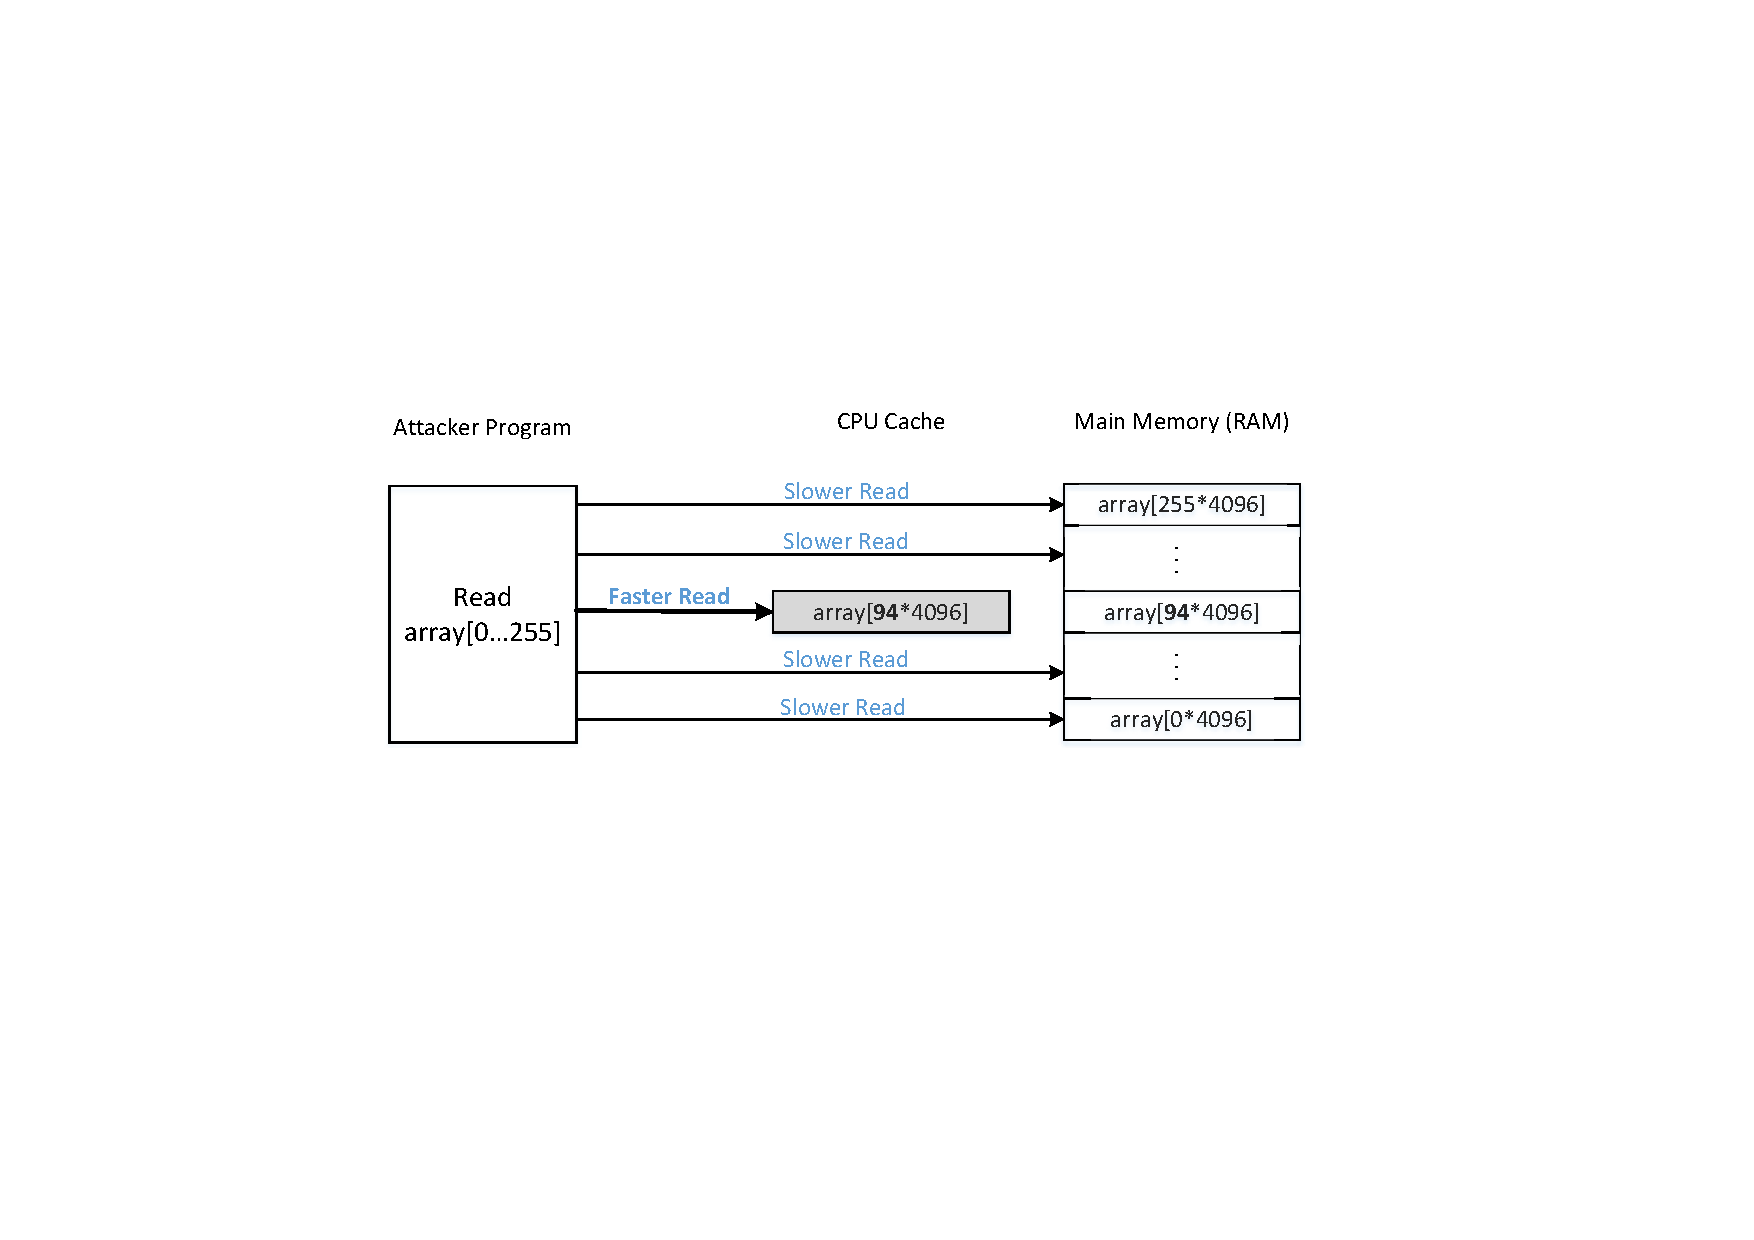
\includegraphics[width=0.9\textwidth]{\sideChannelFigs/flushreload.pdf}
\caption{Diagram depicting the Side Channel Attack}
\label{sidechannel:fig:flushreload}
\end{figure}


The objective of this task is to use the side channel to extract a secret value used by the
victim function. Assume there is a victim  function that uses a secret value as index
to load some values from an array. Also assume that the secret value cannot be accessed from
the outside. Our goal is to use side channels to
get this secret value. The technique that we will be using is called 
FLUSH+RELOAD~\cite{Yarom2014}. Figure~\ref{sidechannel:fig:flushreload} illustrates the 
technique, which consists of three steps: 

\begin{enumerate}[noitemsep]

\item FLUSH the entire array from the cache memory to make sure the array is not cached. 

\item Invoke the victim function, which accesses one of the array
elements based on the value of the secret. This action causes 
the corresponding array element to be cached. 

\item RELOAD the entire array, and measure the time it takes to reload 
each element. If one specific element's loading time is fast, 
it is very likely that element is already in the cache. 
This element must be the one accessed by the victim function. 
Therefore, we can figure out what the secret value is.
\end{enumerate}


The following program uses the FLUSH+RELOAD technique to 
find out a one-byte secret value contained in the variable \texttt{secret}. 
Since there are 256 possible values for a one-byte secret, we 
need to map each value to an array element. The naive way is to define an
array of 256 elements (i.e., \texttt{array[256]}).  However, this does not
work. Caching is done at a block level, not at a byte level. If
\texttt{array[k]} is accessed, a block of memory containing this element  
will be cached. Therefore, the adjacent elements of \texttt{array[k]} 
will also be cached, making it difficult to infer what the secret is. 
To solve this problem, we create an array of \texttt{256*4096} 
bytes. Each element used in our RELOAD step is \texttt{array[k*4096]}. 
Because \texttt{4096} is larger than a typical cache block size (64 bytes), 
no two different elements \texttt{array[i*4096]} and \texttt{array[j*4096]} will
be in the same cache block.

Since \texttt{array[0*4096]} may fall into the same cache block as the variables 
in the adjacent memory, it may be accidentally cached due to the caching 
of those variables. Therefore, we should avoid using \texttt{array[0*4096]} in
the FLUSH+RELOAD method (for other index \texttt{k}, \texttt{array[k*4096]} does not
have a problem).
To make it consistent in the program, we use 
\texttt{array[k*4096 + DELTA]} for all \texttt{k} values, 
where \texttt{DELTA} is defined as a constant \texttt{1024}. 


\begin{lstlisting}[caption=\texttt{FlushReload.c}, label={sidechannel:list:flushreload}]
#include <emmintrin.h>
#include <x86intrin.h>

uint8_t array[256*4096];
int temp;
unsigned char secret = 94;

/* cache hit time threshold assumed*/
#define CACHE_HIT_THRESHOLD (80)
#define DELTA 1024

void flushSideChannel()
{
  int i;

  // Write to array to bring it to RAM to prevent Copy-on-write
  for (i = 0; i < 256; i++) array[i*4096 + DELTA] = 1;


  // Flush the values of the array from cache
  for (i = 0; i < 256; i++) _mm_clflush(&array[i*4096 +DELTA]);
}

void victim()
{
  temp = array[secret*4096 + DELTA];
}

void reloadSideChannel() 
{
  int junk=0;
  register uint64_t time1, time2;
  volatile uint8_t *addr;
  int i;
  for(i = 0; i < 256; i++){
     addr = &array[i*4096 + DELTA];
     time1 = __rdtscp(&junk);
     junk = *addr;
     time2 = __rdtscp(&junk) - time1;
     if (time2 <= CACHE_HIT_THRESHOLD){
         printf("array[%d*4096 + %d] is in cache.\n", i, DELTA);
         printf("The Secret = %d.\n",i);
     }
  }	
}

int main(int argc, const char **argv) 
{
  flushSideChannel();
  victim();
  reloadSideChannel();
  return (0);
}
\end{lstlisting}
 

Please compile the program using \texttt{gcc} and run it (see Section~\ref{sidechannel:sec:compilation}
for compilation instruction).
It should be noted that the technique is not 100 percent accurate, and you may not 
be able to observe the expected output all the time. 
Run the program for at least 20 times, and count how many times 
you will get the secret correctly. You can also adjust the 
threshold \texttt{CACHE\_HIT\_THRESHOLD} to the one derived from
Task 1 (80 is used in this code). 


